%lagrange 文档
\documentclass{xtupaper}
\usepackage[urlcolor=blue]{hyperref}
\usepackage{threeparttable}
\usepackage{setspace}
\usepackage{titlesec}
\usepackage{float}
\newcommand{\upcite}[1]{\textsuperscript{\textsuperscript{\cite{#1}}}}
\usepackage{fancyhdr}
\titleformat{\section}{\large \heiti}{\chinese{section}、}{0em}{}
\begin{document}
	\begin{center}
		\LARGE
		\textbf{数值计算方法---拉格朗日插值法求近似值}\\
		\vspace{0.5em}
		\large
		王艺博,\ PHI1\_NA@outlook.com\\
		湘潭大学,\ 数学与计算科学学院
	\end{center}
	\rule[0.1\baselineskip]{\textwidth}{0.5pt}
	
	
	\section{Lagrange插值法} 
对于$n+1$个样本点$ (x_i,y_i),i=0,1,2,\dots
,n  $
\[L_n(x)=\sum_{i=0}^{n}y_iI_i(x)\]
\[I_i(x)=\frac{(x-x_0)(x-x_1)\dots(x-x_{i-1})(x-x_{i+1})\dots(x-x_n)}{(x_i-x_0)(x_i-x_1)\dots(x_i-x_{i-1})(x_i-x_{i+1})\dots(x_i-x_n)}\]

$ L_n(x) $为$ f(x) $的n次多项式插值的Lagrange公式,也称为Lagrange插值多项式

\[I_i(x)=\frac{\omega_n(x)}{(x-x_i)\omega_n'(x_i)}\]

$ I_i(x) $称为n次多项式插值问题的基函数(Lagrange因子),其中
\[\omega_n(x)=\prod_{j=0}^{n}(x-x_j)\]
\newpage
	\section{算法}
	
	$\heartsuit$ Lagrange插值法:\verb|  [y] = Lag_interp_v1(x0,y0,x)|
	
	\paragraph{输入:} 
	
	\begin{itemize}
		\item  已知插值点的横坐标向量 $x0$,
		
		\item 已知插值点的纵坐标向量 $y0$,
		
		\item 所求点的横坐标向量 $x$,
		
	\end{itemize}
	
	\paragraph{输出:}
	\begin{itemize}
		\item 所求点的近似值对应的向量 $y$.
	\end{itemize}

	
	\paragraph{实现步骤:}
	
	\begin{itemize}
		\item 步骤 $1$: 输入x0,x	
		\item 步骤 $2$: 计算每个$ x $对应的 Lagrange基函数 $ I_i(x) $
		\item 步骤 $3$: 输入y0
		\item 步骤 $4$: 结合 $I_i(x) $与$ y0 $ 计算每个x对应的$ Ln(x) $
		\item 步骤 $5$: 输出对应的$ Ln $
	\end{itemize}
\begin{figure}

	\begin{algorithm}[H]
		\caption{ Lag\_interp\_v1 思路}
		\label{alg:Framwork}
		\begin{algorithmic}
			\State 输入:插值点向量$x0$, 插值点向量 $y0$, 所求点向量$x$
			
			\State 输出:所求点Lagrange近似值向量$Ln$
			\newline
			\State 设n1,n2
			
			 n1 表示插值点的个数;
			
			n2 表示所求点的个数;
			
			\State 计算一个$x(j)$对应的基函数中的一项$I(i)$;
			
			将下式中的$ x $看成$ x(j) $
			\[I_i(x)=\frac{(x-x_0)(x-x_1)\dots(x-x_{i-1})(x-x_{i+1})\dots(x-x_n)}{(x_i-x_0)(x_i-x_1)\dots(x_i-x_{i-1})(x_i-x_{i+1})\dots(x_i-x_n)}\]
			
			\State 使用 if 和 prod内置函数 来实现 $ I_i(x) $的表示
				
				 prod 表示矩阵中所有元素的乘积
				
				构建这样的矩阵  \[ omega\_x =[x(j)-x0_1,x(j)-x0_2,x(j)-x0_3\dots,x_j-x0_{n1}] \]
				
				利用程序中矩阵的运算,表示为 数 与 向量的相减
				\[ x(j) - x0 = omega\_x\]
				
				使用$ prod(omega\_x[1:i-1,i+1:n1]) $表示$ I_i(x) $分子
				
				同理,使用 prod 表示$ I_i(x) $分母
				
				考虑到$ i-1 $ 与$ i+1 $分别在$ i=1 $与$ i=n1 $时$ omega\_x(0) $与$ omega\_x(n1+1) $无意义
				
				使用 if 对其进行单独讨论
			\State\textbf{if} i == 1
			
					$ I(i) = prod(omega\_x(i+1:n1))/prod(w(i+1:n1)); $
					
			\State \textbf{elseif}  i == n1
 			
				$ I(i) = prod(omega\_x(1:i-1))/prod(w(1:i-1)); $
			\State \textbf{else}
			    
			    $I(i) = prod(omega\_x(1:i-1))/prod(w(1:i-1)); $
				
				$ I(i) = I(i) * prod(omega\_x(i+1:n1))/prod(w(i+1:n1)); $
			\State \textbf{end}
			\State 对上述$ I_i(x) $
			\State\textbf{for} $ i = 1:1:n1 $
			
			得到 对于一个$ x(j) $的 \[I= [I_1(x),I_2(x),\dots,I_{n1}(x)]\]
			
			\State 对于 $ x(j)   $\quad$ Ln(x) = y0*I^T $

			
			\State \textbf{for} $ j =1:1:n2 $
			\State 得到每一个 x 的 I
			
			\State 最终\\输出得到向量$ Ln $
				  
			
		\end{algorithmic}
	\end{algorithm}
\end{figure}
	\newpage
	\section{北太天元源程序}
	\begin{lstlisting}[language=matlab]
	%Lagrange 插值公式
	%  x0:样本点横坐标所构成的行向量
	%  y0:样本点纵坐标所构成的行向量
	%  x :所求点的横坐标,所构成的行向量
	%  y :得到所求点纵坐标,构成行向量
	%函数使用时,需要在命令行中输入pwd或cd 进入函数所在的文件夹
function  [y] = Lag_interp_v1(x0,y0,x)
		n1 = length(x0);   % n1表示样本点的个数 
		I = zeros(1,n1);   % 预留出要用的空间
		n2 = length(x);	   % n2表示所求点的个数
		Ln = zeros(1,n2);
	for j=1:1:n2    	%  依次代入 自变量 x(j) 
		omega_x = x(j)-x0;    % 数 - 矩阵 ,表示 [x(j) - x0(1),x(j)-x0(2),...,x(j)-x0(n1)]
		for i = 1:1:n1   %  对于x(j)求对应的基函数 I(i)
			w = x0(i) - x0;  % 同样是 数 - 矩阵
				% 这里使用 if 和 内置的 prod 函数代替了 for 循环
				% prod 表示矩阵内所有元素的乘积
			if i == 1	
				% omega_x(i+1:n1)表示向量的节选,第i+1个到第n1个元素
				I(i) = prod(omega_x(i+1:n1))/prod(w(i+1:n1));
			elseif i == n1
				I(i) = prod(omega_x(1:i-1))/prod(w(1:i-1));
			else
				I(i) = prod(omega_x(1:i-1))/prod(w(1:i-1));
				I(i) = I(i) * prod(omega_x(i+1:n1))/prod(w(i+1:n1));
			end 
		end
		%使用矩阵的乘积,行向量 × 列向量 得到一个值
		Ln(j) = y0*I'; 
	end	
	y = Ln;
end
	\end{lstlisting}
	将上述代码保存为\verb|Lag_interp_v1.m|文件。
	\newpage
	\section{数值算例}
	\begin{example}\label{exmJacobi1} 
利用$ f(x) = ln x $的如下数据:

\begin{center}% 居中环境
	\begin{tabular}{|c|c|c|c|c|}
		\hline
		x & 0.4 & 0.5 & 0.6 & 0.7 \\
		\hline
		ln x  & -0.916291 & -0.693147 & -0.510826 & -0.357765 \\
		\hline
	\end{tabular}
\end{center}
进行Lagrange插值;
\begin{enumerate}
	\item 计算 x = [0.412 0.511 0.666] 处的近似值
	\item 计算$ x_i = 0.3 + ih,h=0.01,i = 0,1,2,\dots,50 $处的近似值,并作图

\end{enumerate}
	\end{example}
	
调用函数 \verb|[y] = Lag_interp_v1(x0,y0,x)|,相应的实现代码为:
	\begin{lstlisting}[language=matlab]
	clc, clear all, format long;
	x0 = linspace(0.4,0.7,4); % 输入样本点的横坐标
	y0 = [-0.916291 -0.693147 -0.510826 -0.35765]; % 输入样本点的纵坐标
	% 简单的算几个点
	x1 = [ 0.412 0.511 0.666];
	y1 = Lag_interp_v1(x0,y0,x1);
	for i = 1:1:length(x1)
		fprintf('f(%f) = %f \n',x1(i),y1(i));
	end
	% 利用很多的点来画图
	x2 = linspace(0.3,0.8,51); % 共51个要求的点
	% 利用写好的 Lag_interp_v1 函数计算要求点的纵坐标
	y2 = Lag_interp_v1(x0,y0,x2);
	delta = abs(y2-log(x2));
	%作图
		figure(1); %画出第一个图像
		plot(x2,y2,'b');

		figure(2);
		plot(x2,y2,'b');
		hold on
			plot(x2,log(x2),'r'); % y = lnx 的图像
		hold off
	%Ln(x) 与 lnx 的 误差 
		figure(3); % 画出第二个图像
		plot(x2,delta,'g');
	% 文字形式表示出来
	for j = 1:1:51
		fprintf('f(%f) = %f \n',x2(j),y2(j));
	end
	\end{lstlisting}
	将上述代码保存为 \verb|LagTest.m|
	
	在北太天元软件的命令行窗口输入:
	\begin{lstlisting}
		>> LagTest
	\end{lstlisting}
	回车可得运算结果
	\begin{lstlisting}
	f(0.412000) = -0.886972 
	f(0.511000) = -0.671305 
	f(0.666000) = -0.407185 
	f(0.300000) = -1.191936 
	f(0.310000) = -1.161676 
	f(0.320000) = -1.132046 
	f(0.330000) = -1.103035 
	f(0.340000) = -1.074630 
	
	此处省略

	f(0.770000) = -0.261515 
	f(0.780000) = -0.248246 
	f(0.790000) = -0.235059 
	f(0.800000) = -0.221941 
	\end{lstlisting}
	
	\iffalse
	\begin{table}[htp]
		\caption{表格}
		\centering
		\begin{tabular}{cccccccc}
			\toprule[1.5pt]
			年份  & 2006&2007&2008&2009&2010 & 2011 & 2012 \\
			\midrule
			A&57.95&58.187&59.1&59.652&60.22&61.072&61.418 \\
			B &55.7957 &58.3199&58.8548&59.9983&60.3769 &60.9841 &61.7716 \\		
			C&2.1543&0.1329&0.2452&0.3463&0.1569&0.0879&0.3536 \\		
			D&0.0372 &0.0023&0.0041&0.0058&0.0026&0.0014&0.0058 \\
			\bottomrule[1.5pt]
			\label{tab1}
		\end{tabular}
	\end{table}
	\fi
	\begin{figure}[htp]%H表示图强制在下面,想设置浮动环境用htp
		\centering  %插入的图片居中表示
		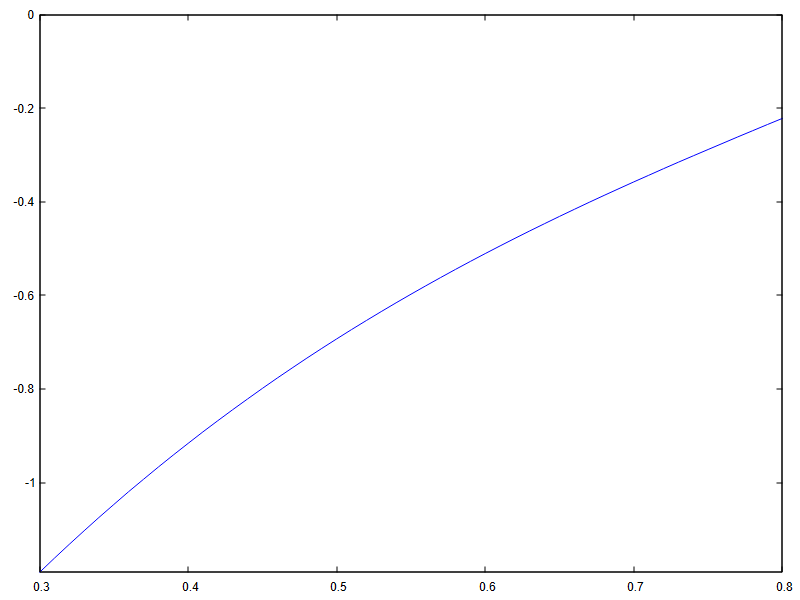
\includegraphics[scale=0.5]{graph1} 
		\caption{$ L_n(x) $的图像}  %图片的名称
%		\label{figSol}
	\end{figure}
	
	\begin{figure}[htp]%H表示图强制在下面,想设置浮动环境用htp
		\centering  %插入的图片居中表示
		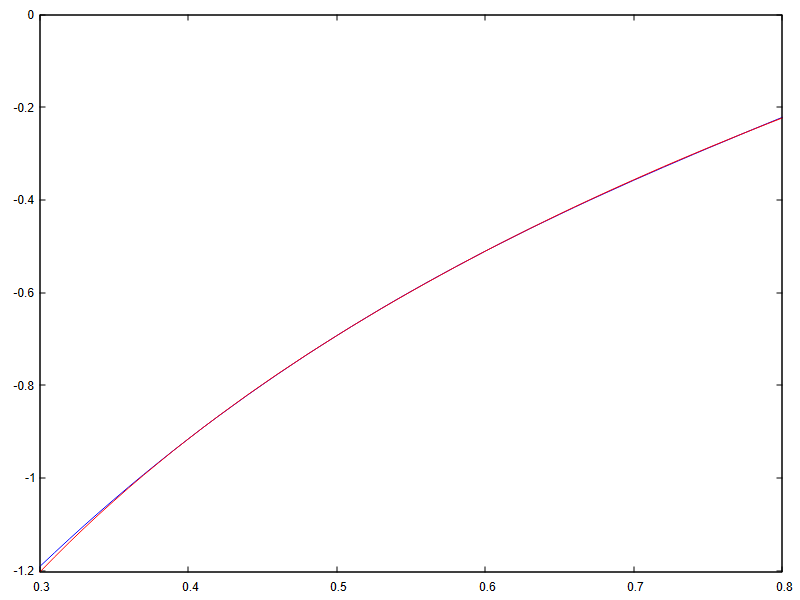
\includegraphics[scale=0.5]{graph2} 
		\caption{$ L_n(x) $与 $ ln(x) $的图像}  %图片的名称
%		\label{figRes}
	\end{figure}
	
	\begin{figure}[htp]%H表示图强制在下面,想设置浮动环境用htp
		\centering  %插入的图片居中表示
		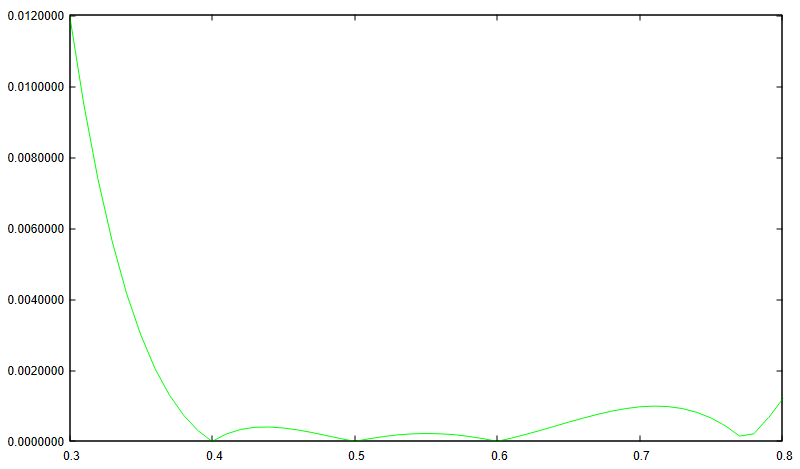
\includegraphics[scale=0.5]{graph3} 
		\caption{$ L_n(x) $与 $ ln(x) $的误差}  %图片的名称
%		\label{figErr}
	\end{figure}
	
\end{document} 
